%!TEX root = ./main.tex
\section{Introduction}

\subsection{A brief overview of Phase Contrast}
\begin{wrapfigure}{L}{0.45\textwidth}
    %\begin{figure}[!b]
        \centering
       % \begin{minipage}{0.6\textwidth}
            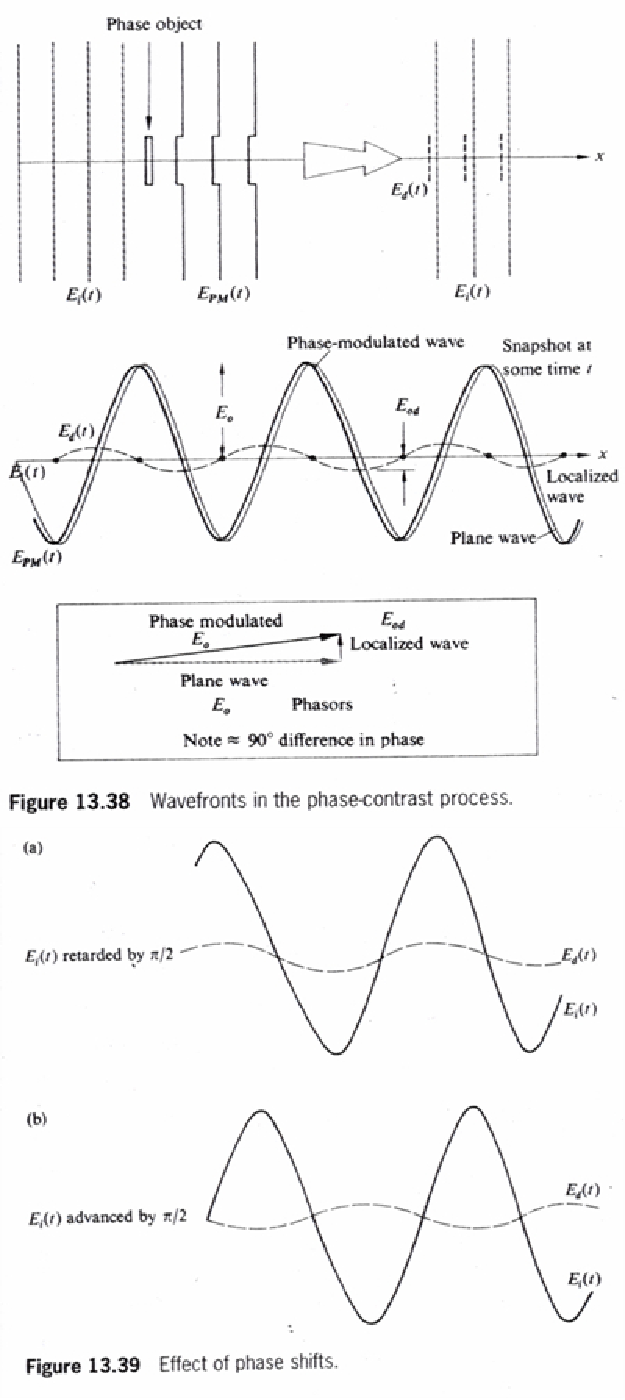
\includegraphics[width=0.45\textwidth]{figures/phasediff.pdf}
            %\captionsetup{margin={0pt,0.6\textwidth},width=\textwidth}
            \caption{Wavefronts in phase contrast process (image credit `Optics by Eugene Hetch')}
            \label{fig:hetchphase}
       % \end{minipage}
    %\end{figure}
\end{wrapfigure}


Phase contrast microscopy has been around for quite a while.
While it has revolutionized the world of optical microscopy, it also provided interesting insights into physics of imaging in itself.
Whenever any nearly `transparent' object scatters any incoming wave, it leaves the amplitude of the wave more or less intact, however phase of the incoming wave is altered very slightly.
This small advancement or retardation of phase results in difference of $\pi/2$ between the 2 waves(Figure~\ref{fig:hetchphase}).
Usually this phase difference will not make any noticeable change in contrast, but if incident or scattered wave is modulated by extra phase of $\pi/2$. then this phase contrast can be converted to amplitude contrast.
This is the fundamental principle behind phase contrast microscopy.

There is another method to extract information of phase from the image object, that is `holography'. 
Basic idea behind holograhpy is to record an interferogram between scattered wave and incident wave, this way all of the information of original scattering object is retained in single interferogram or hologram.
Holography, for our interest here, can be divided in roughly 2 segments:
\textbf{Inline} and \textbf{Off-axis} holography.
Inline holograhpy was first described by D. Gabor in 1948.\cite{Gabor1948}.
In Inline holography, scattered waves from an object interfere with unscattered waves from the same source to produce hologram.
While in Off-axis holography, incoming beam is first split into two beams, one of which then interacts with the object, after which it interferes back with the other half (the unscattered wave) to produce the hologram.

\begin{wrapfigure}{L}{0.5\textwidth}
    \centering
    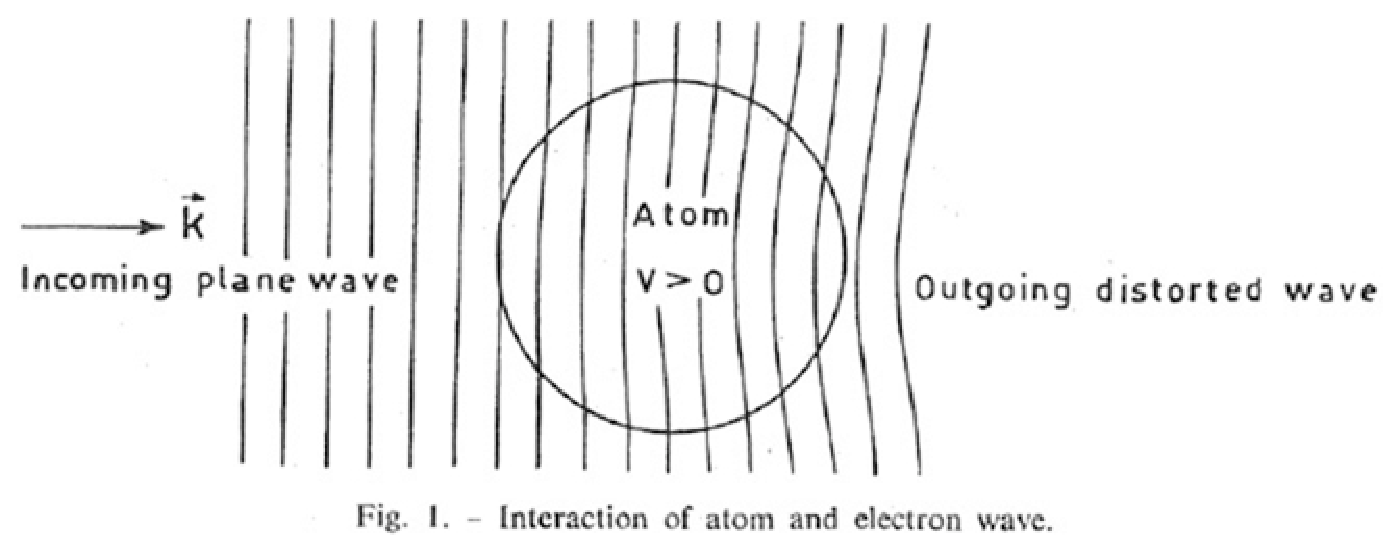
\includegraphics[width=0.5\textwidth]{figures/electronphase.pdf}
    \caption{Electron plane wave retardation by an atom (image credit: unknown)}
    \label{fig:electronphase}
\end{wrapfigure}

The high resolution electron microgram, produced from highly coherent field emission source, is an inline hologram.
Hence it not only contains information about the position of particles but their relative phases as well.
When an electron plane wave passes through an atom, due to the positive potential at the core atom, phase of electron waves advances slightly (Figure~\ref{fig:electronphase}).
Hence now the distorted electron plane wave carry information about not only position of atoms (relative phases with respect to each other), but also of atomic number of the atom (magnitude of phase change).
This information if extracted can elucidate entire structure of any given sample.
This as formed image of the sample on the plane wave of electron is called `Exit Wave'.

Problem for electron microscopy is complicated slightly by the lens aberrations.
As we shall see shortly phase of electron plane wave in an electron microscope depend on the defocus value and aberration coefficients of the electron microscope.
Hence to reconstruct our original object we have to deconvolute effects of both defocus and aberrations from our images to obtain pure exit wave.
To understand effects of aberrations on the image, first we need to have a look at the transfer function of electron microscope.


\subsection{Effects of Defocus and Spherical Aberration}
We shall discuss effects of two defects in image which do not originate from sample ($k$-spacing) or from physical limitations of electron beam (\textit{e.g.} decoherence and $\lambda$), \textit{i.e.} defocus and spherical aberration.

\begin{figure}
    \centering
    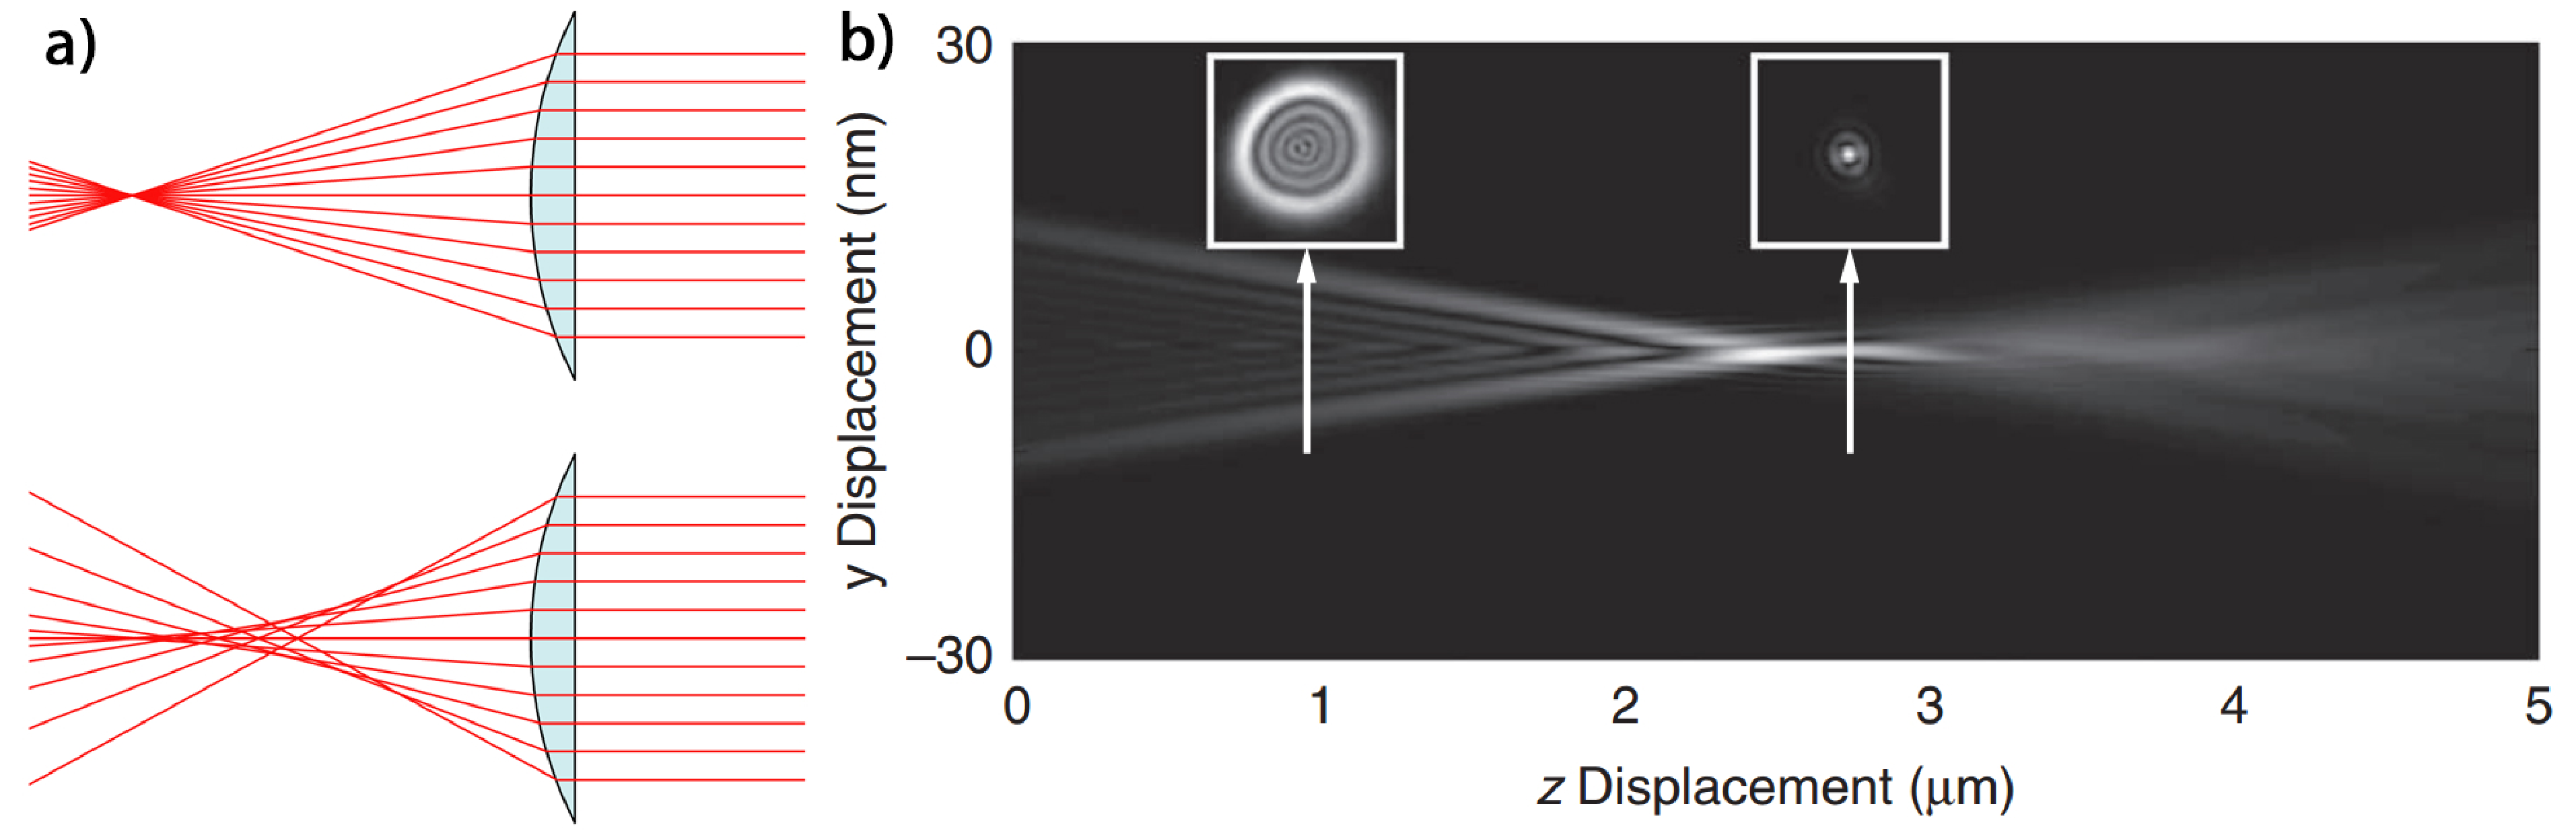
\includegraphics[width=\textwidth]{figures/circleleastconf.pdf}
    \caption{a) Simple diagram showing perfect lens with point focus and lens with spherical aberration, and b) Probe size at different defocus values for a source focused with lens having spherical aberration (Ref \cite{Humphry2012})}
    \label{fig:leastconfusion}
\end{figure}

\textbf{Defocus} is simply defined as the difference between the plane in which currently lens is focusing as opposed to the plane in which lens shall focus ideally.
Focal length of lens is essentially the point where image of a point is reproduced as a point.
Any lens with any defect in it will not reproduce image of a point as a point but rather as `spread', whose precise form is determined by the Point Spread Function (PSF) of the lens.
If a lens has no other defect but just defocus, then its PSF can be described mathematically as a simple Gaussian function.


\textbf{Spherical Aberration:} Spherical aberration is the defect in optics when rays, coming from different part of of lens (from the edge of the lens as compared to near axis of lens) focuses at different positions long principal axis, as shown in Figure~\ref{fig:leastconfusion}a (when it focus at same value of principal axis but at different positions in plane $\bot$ to lens plane, then it is called `Coma').
Because of spherical aberration PSF of a point is now rather represented as a disk.
The smallest of such disk which is created by spherical aberration is called `Circle of Least Confusion', as that is sharpest image that could be produced of a point (Figure~\ref{fig:leastconfusion}b).
As pointed out by Scherzer\cite{Scherzer1949}, due to cylindrical symmetry of EM lenses and the fact that EM lenses can only be converging, (magnetic field is always stronger at edges as compared to the center of lens hence it can only converge the electron beam) all EM lenses contains inherent spherical aberration (in optics spherical aberration is corrected by diverging lenses to compensate for the difference in focal lengths).
\footnote{For correcting spherical aberration, lenses were needed which were not cylindrically symmetric. Among other ideas such as lenses with charged axis etc, multipolar lenses were suggested (see \cite{Rose2009} for detailed discussion).
In 1997 first successful practical aberration corrected TEM was reported using hexapole correctors \cite{Haider1998}, followed by an independent report using quadrapole/octapole correctors \cite{Batson2002}.
Aberration correction by the use of multipole unsymmetrical lenses will not be discussed any further.}

In fourier optics, as discussed earlier image formation can be described as the convolution of PSF of the lens on to the perfect image of object  to be imaged.
In case of TEM it would be convolution of PSF of objective lens on to the exit wave of sample.
Point spread function of TEM is rather complex and is discussed in detail in following section.


\subsection{Contrast Transfer Function}
Transfer functions are described as mathematical functions of and `response' given from any instrument. 
That is, as in the case of TEM, the function mapping the outgoing exit wave (electron lane wave after interacting with the sample) to the observed contrast or image.
As image formation is done by objective lens, in above case it will be the transfer function of the objective lens, \textit{i.e.}
\begin{equation}
    \psi_t(x) = t(x) \psi_{inc}(x)
    \label{eq:exitwave1}
\end{equation}

where: 
\begin{description}
    \item[\psi_{inc}(x)] = incident plane wave
    \item[t(x)] = transmission function (ie how, for different `x', $\psi_{inc}(x)$ is modified after transmission from sample)
    \item[\psi_t(x)] = exit plane wave, i.e electron plane wave just after passing through the specimen
\end{description}

Effects of lens aberrations on $\psi_{t}(x)$ is to shift intensity of it as a function of aberrations and spatial frequency (lattice spacing of various planes).
Effects of such aberrations can be represented mathematically as the convolution operator.

\begin{equation}
    \psi_i(x) = \psi_t(x) \ast h_o(x)
    \label{eq:imgplnconv}
\end{equation}

where:
\begin{description}
    \item[\psi_i(x)] = image plane wave
    \item[\ast] denotes convolution operator
\end{description}  

In fourier space it can be written as:
\begin{align*}
    FT\{\psi_i(x) = \psi_t(x) \ast h_o(x)\}
\end{align*}
\begin{equation}
    \Psi_i(\boldsymbol{k}) = \Psi_t(\boldsymbol{k}) . H_o(\boldsymbol{k})
    \label{eq:fourierconv}
\end{equation}
That is because, convolution operator in real space is multiplication in fourier space.
Here $H_o(\boldsymbol{k})$ can be described as:
\begin{equation}
    H_o(\boldsymbol{k}) = exp(-i\chi(\boldsymbol{k}))
\end{equation}
where $\chi(\boldsymbol{k})$ is `Wave Aberration Function' which can be described as:
\begin{equation}
    \chi = 0.5 \pi C_s k^4 \lambda^3 + \pi \Delta f k^2 \lambda + \pi \Delta f_a cos(2(\theta - \theta_c)) k^2 \lambda + \textnormal{higher order terms}... 
\end{equation}

Here:
\begin{description}
    \item[C_s] = Spherical aberration coefficient of the Objective lens
    \item[\Delta f] = average defocus
    \item[\Delta f_a] = variation in defocus due to 2-fold astigmatism
    \item[\theta_c] = angle of astigmatism w.r.t x-axis
\end{description}

Higher order terms include aberrations such as three fold astigmatism, coma, and higher order spherical aberration etc.
For non-aberration corrected TEMs $C_s$ and two fold astigmatism overwhelms other aberrations, hence they shall be focus for now.
Higher order aberrations does show noticeable image degradation in aberration corrected TEMs.

According to weak phase approximation\cite{Scherzer1949}, sample is so thin that it does not affect the amplitude of the electron beam, rather only shifts its phase.
This approximation is valid depending upon 2 things mainly i) sample thickness and ii) atomic number of sample.
While weak phase approximation may remain true for C film for over few nanometers easily, a single uranium atom can invalidate the assumptions.
If weak phase approximation is held true then only above phase difference will be the contrast contributing member HRTEM images.
In such case only complex part of $H_o(\boldsymbol{k})$ is of any interest.
Hence, neglecting higher order terms, and assuming sample to be weak phase object, transfer function can simply be written as $sin$ function or:
\begin{equation}
    T(k) = -sin(\frac{\pi}{2}C_s \lambda^3 k^4 + \pi \Delta f \lambda k^2)
    \label{eq:ctf}
\end{equation}

Therefore it can be stated that information represented in TEM image is controlled by two factors, namely i) Spherical aberration ($C_s$) and ii) defocus ($\Delta f$)
Besides $C_s$, coherency of beam also affects the transfer function of the TEM.
Spatial decoherence of electron plane wave results in formation of an envelope function which reduces contrast at higher spatial frequencies.
Envelope function for coherence ($E_c$) can be represented as :
\begin{equation}
    E_c = e^{|\nabla\chi|^2\beta^2/(4\lambda^2)} e^{-\pi^2\lambda^2d^2 k^4/2}
    \label{eq:chromatic}
\end{equation}
Here:
\begin{description}
    \item[\beta] = convergence angle of beam
    \item[d] = defocus spread due to chromatic aberration 
\end{description}
Contrast Transfer Function or CTF of TEM can now be described as the product of the actual transfer function (Equation~\ref{eq:ctf}) and envelope function (Equation~\ref{eq:chromatic}).
Here the value at which CTF converges to zero is call Information Limit of the microscope.
\begin{figure}[t]
    \centering
    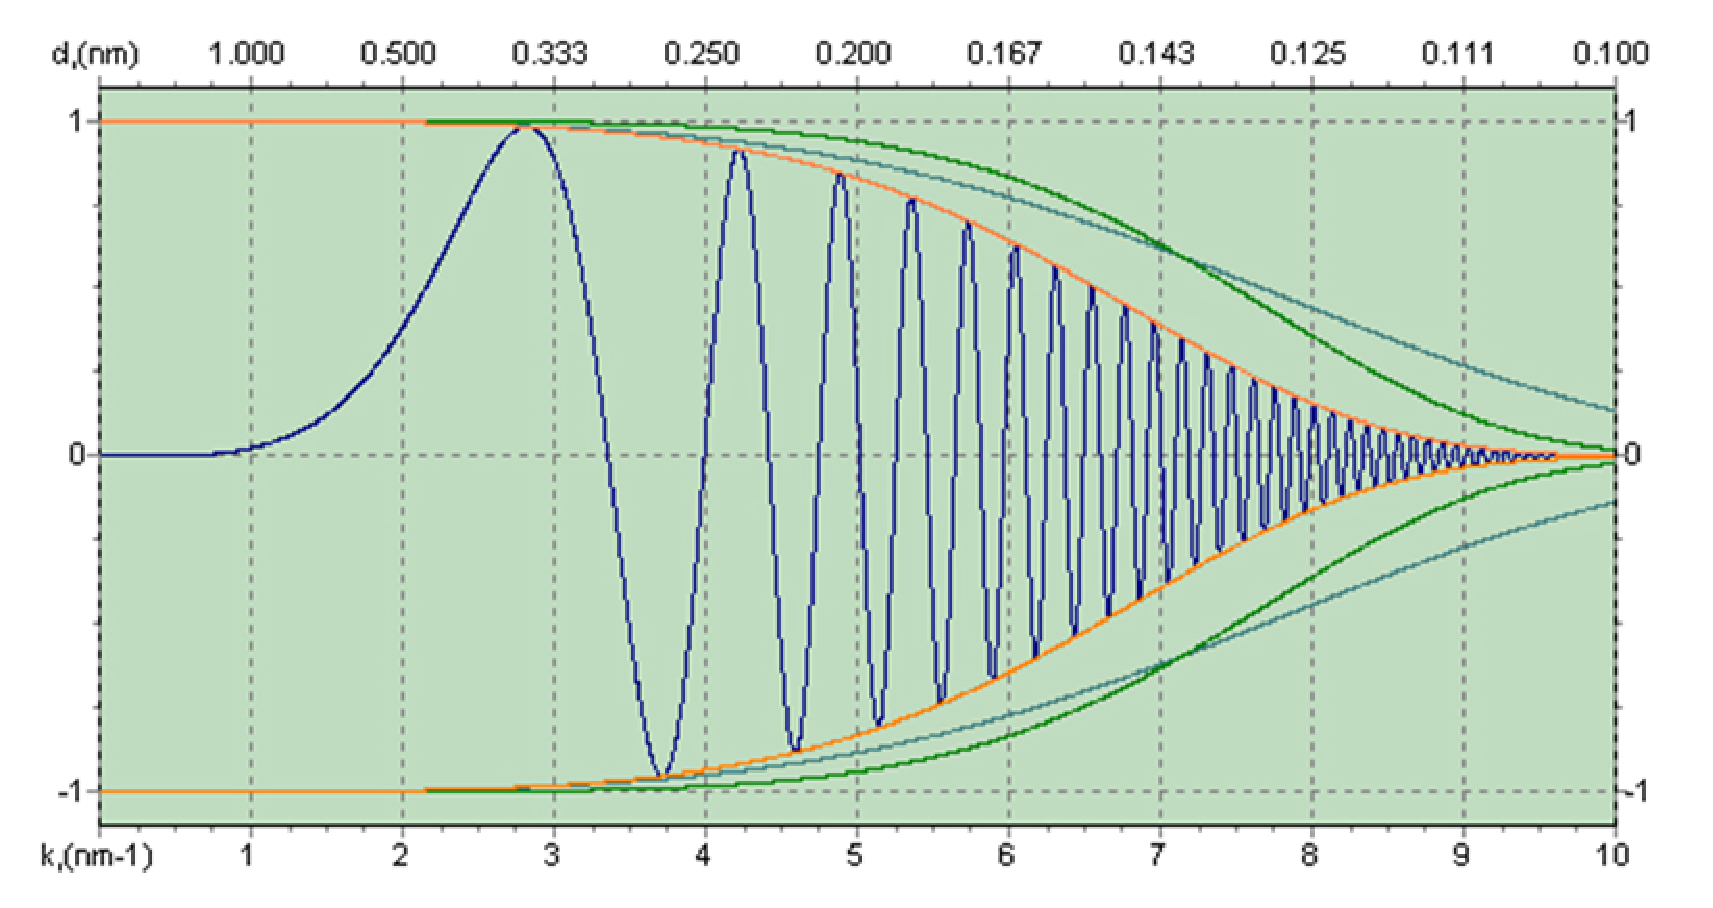
\includegraphics[width=0.8\textwidth]{figures/ctf.pdf}
    \caption{Contrast Transfer Function of TEM (Blue), orange line represents the envelope function}
    \label{fig:ctffigure}
\end{figure}


\begin{wrapfigure}{L}{0.45\textwidth}
    \centering
        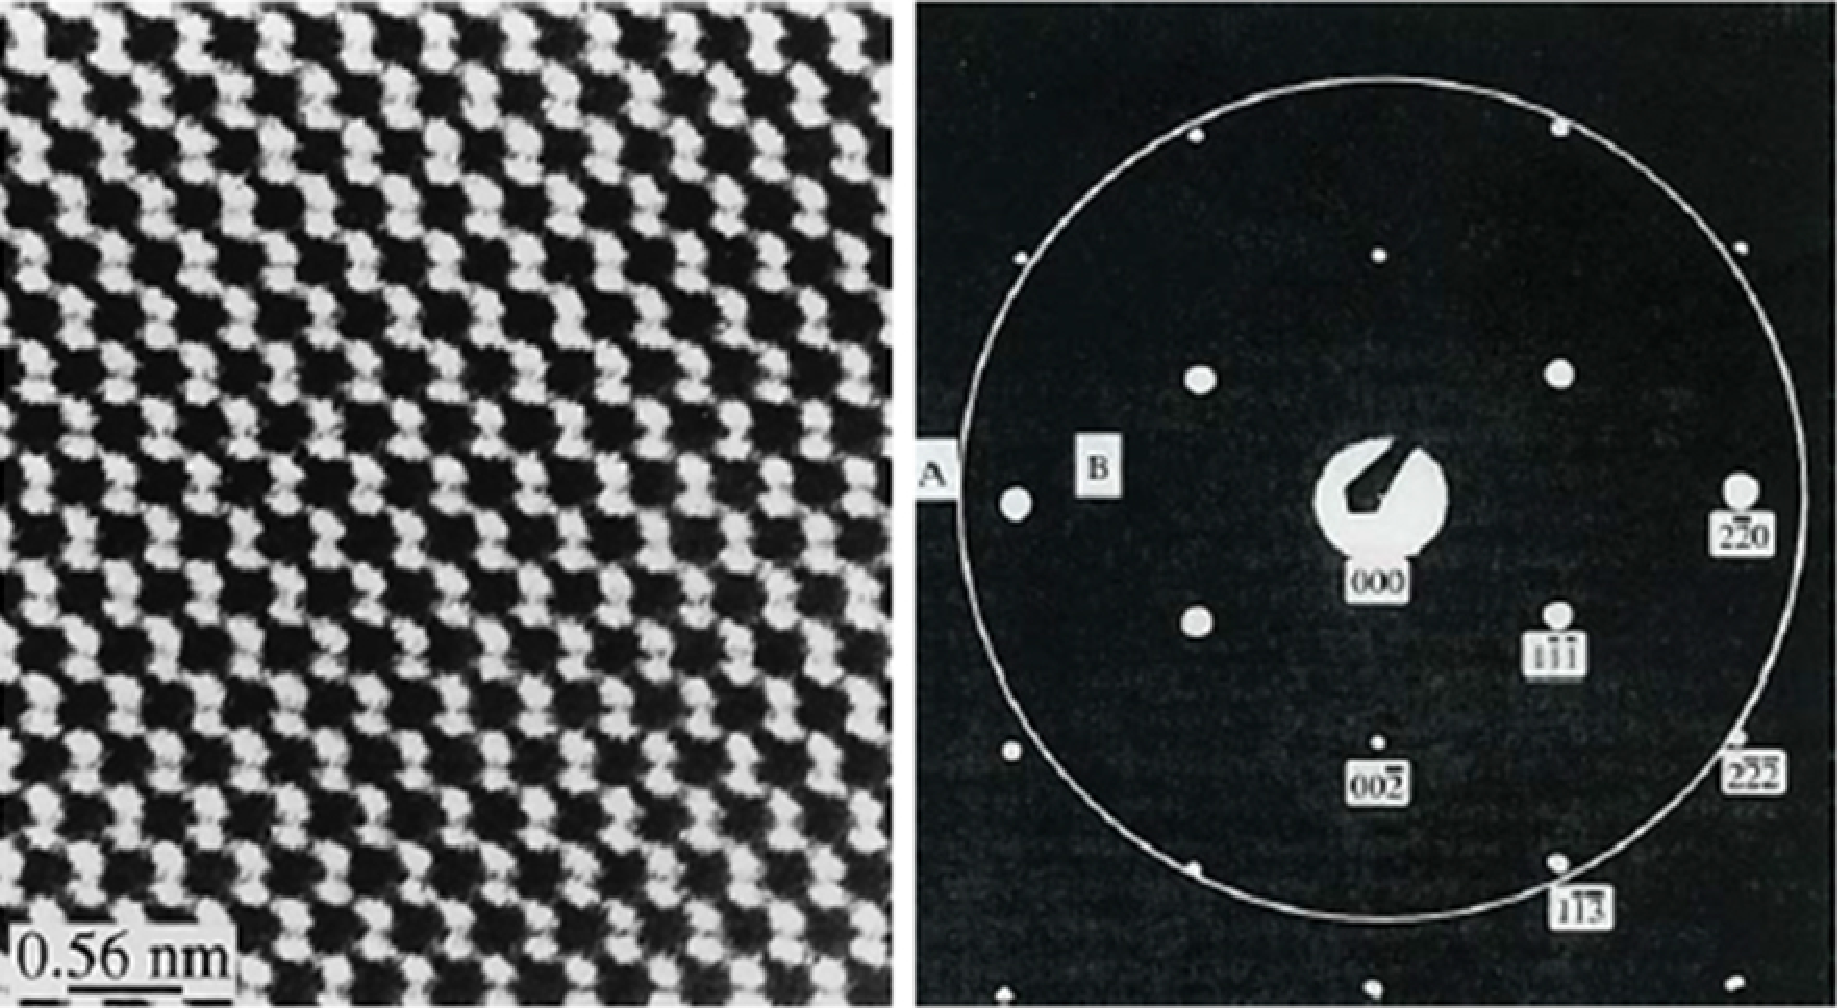
\includegraphics[width=0.45\textwidth]{figures/siwrong.pdf}
        \caption{HRTEM image showing Si `dumbbells' which were mistakenly  identified as from $d_{004}$ lattice}
        \label{fig:siwrong}
\end{wrapfigure}


Figure~\ref{fig:ctffigure} shows CTF vs $k$ plot.
As it is evident, CTF for TEM is not linear but sinusoidal.
Hence depending upon the lattice spacing, in any given image, some lattice planes might appear dark while others might appear light or may not appear at all (zero transfer of contrast).

This makes direct interpretation of HRTEM images rather difficult because TEM image is now complex interference pattern of various lattice spacings of varying intensity. 
At this point any attempt to find position of any atoms present or any direct measurement of lattice constants etc can be severely misguiding.

Shown here in Figure~\ref{fig:siwrong} is one such TEM image where the appearance of `dumbbells' in Si HRTEM was identified as atoms from $d_{004}$ lattice fringes.
Actual fringe spacing of Si $d_{004}$ is 0.14nm and measured $d$-spacing was 0.013nm, leading to the confusion.
It shall be noted that not only microscope resolution limit was much lower, 0.25nm, but at time of image capture objective aperture was masking the $d_{004}$ spot (shown Figure~\ref{fig:siwrong} diffraction pattern with a white ring).
Ultimately that dumbbells were assigned to interference pattern from $d_{113}$ fringes.
This illustrates the difficulties and pitfalls in directly correlating HRTEM intensities with spatial positions of atoms.\footnote{It is often repeated advice that in HRTEM image is forming from interference of various lattice spaces, hence they do not represent true position of atomic columns. An interesting take against this advice can be read here [https://publications.lbl.gov/islandora/object/ir\%3A122777/datastream/PDF/view] by Prof Micheal A. O'Keefe. 

There author mainly discusses how under correct conditions intensities on TEM image does indicate presence of atomic columns, hence incorrect imaging conditions shall not be the reason to say the above statement about atomic positions.}


Other than variation in intensities as described above, spherical aberration also degrades images in one more way, it is called threading.
As spherical aberration focuses electrons nearer to edge of lens more, electron which are scattered the most, with higher $k$ value or low $d$-spacing are focused first.
\begin{figure}
    \centering
    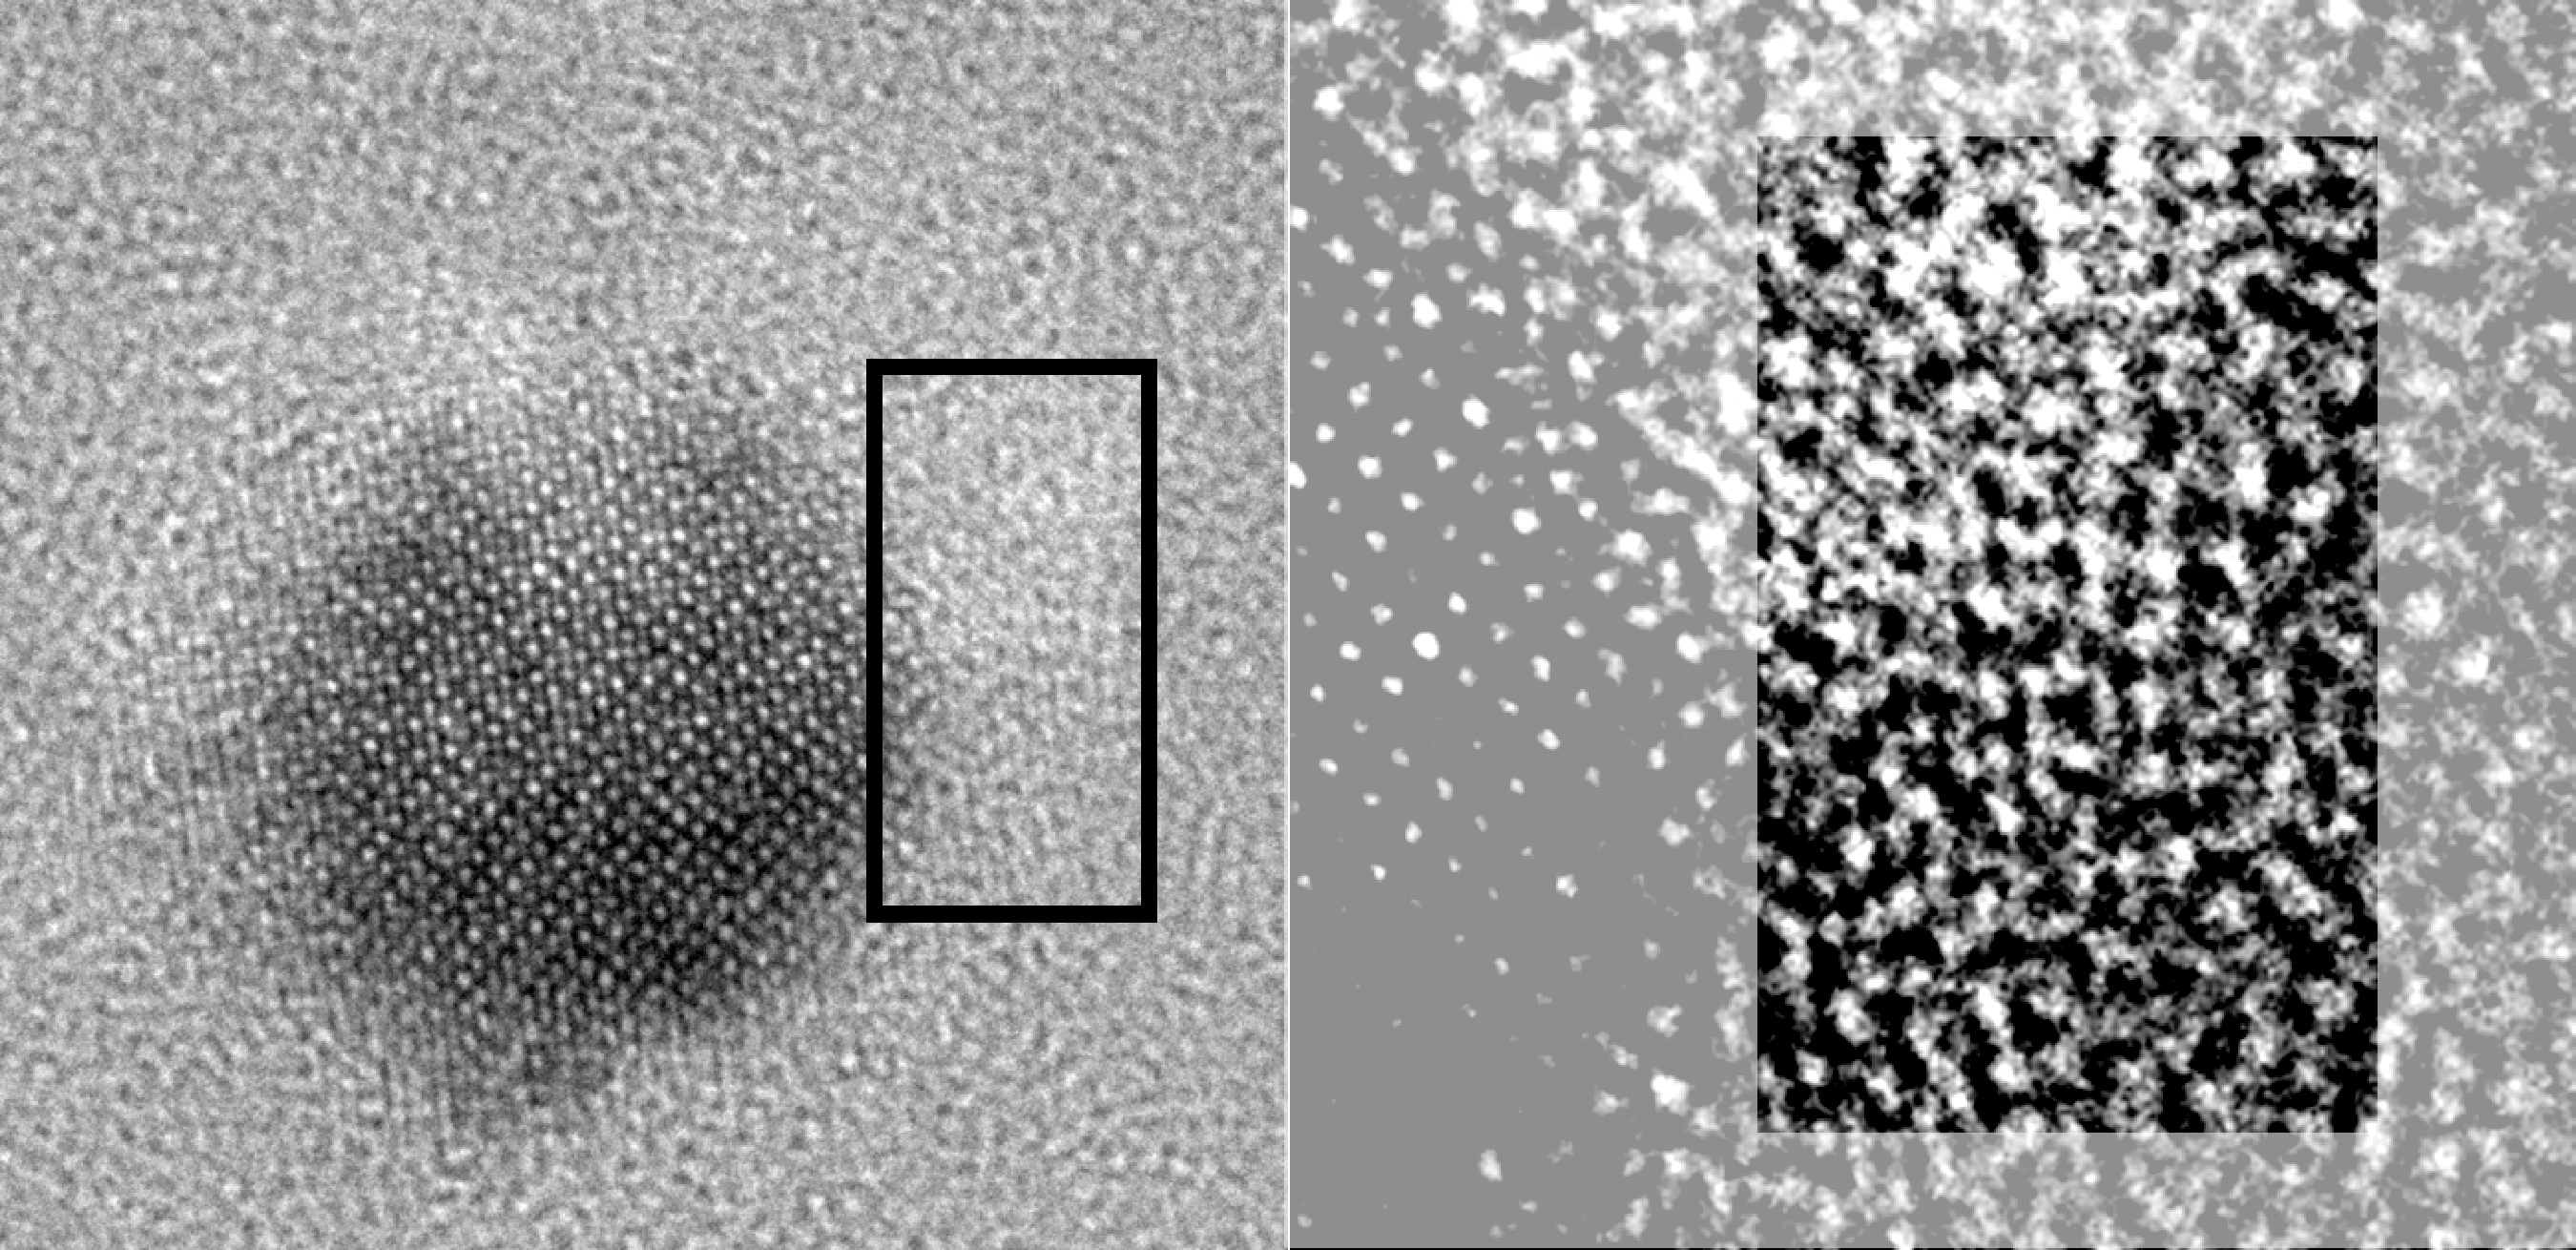
\includegraphics[width=0.8\textwidth]{figures/threading2.pdf}
    \caption{Image showing HRTEM of an Fe\textsubscript{2}O\textsubscript{3} nanoparticle with image intensity from higher $k$ vector, in focus outside boundary of nanoparticle highlighted(right)}
    \label{fig:fe2o3}
\end{figure}
Hence at the exact focus when circle of confusion is least, lattice with higher $k$ values are spread around and form an image away from where it should be located if image intensities were spatially correct (\textit{e.g.} see Figure~\ref{fig:fe2o3}).
This spreading of intensities is called Threading.

This also shows that for a field emission microscope, where beam coherence, and hence consequently, information limit, is large, information for higher $k$ vector or lower lattice spacings is still present in the image.


\begin{wrapfigure}{L}{0.5\textwidth}
    \centering
        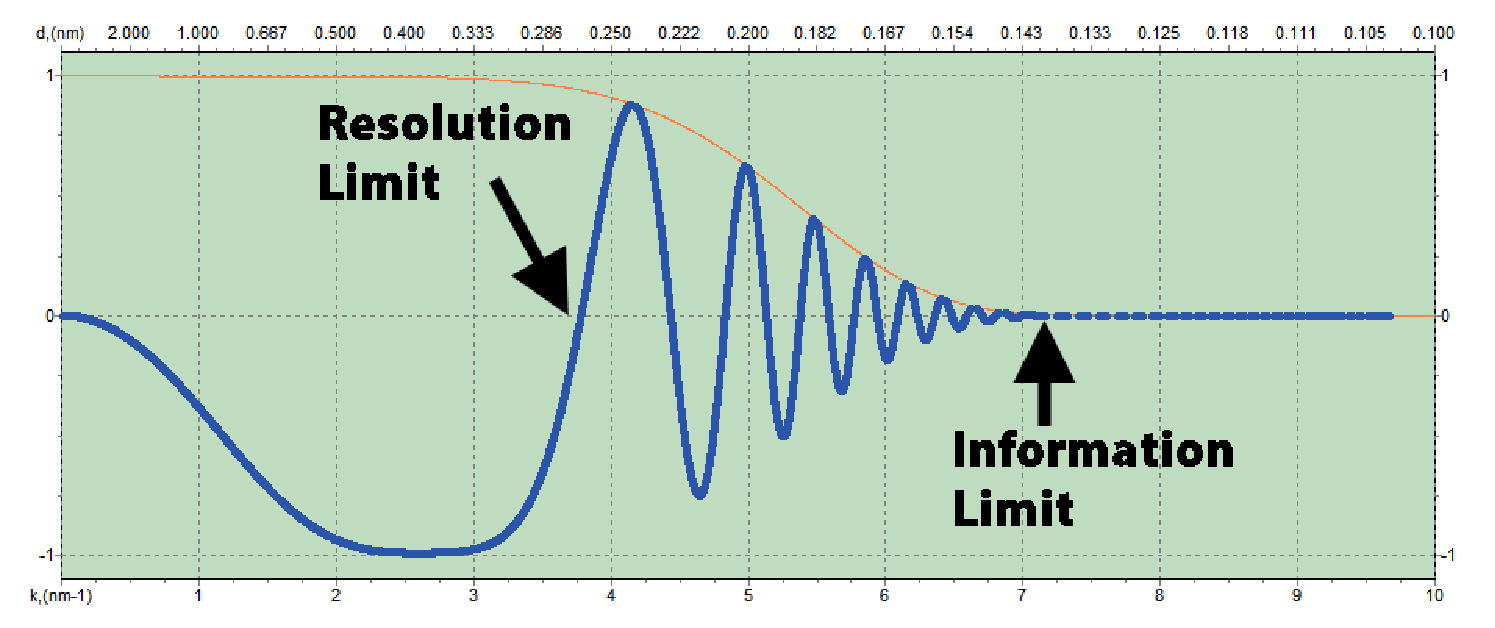
\includegraphics[width=0.5\textwidth]{figures/scherzer.pdf}
        \caption{Image showing CTF of a TEM at Scherzer defocus, with arrows to indicate resolution and information limit}
        \label{fig:ctfsherz}
\end{wrapfigure}


\subsection{Resolution Limit and Defocus} 

Resolution limit of any electron microscope is defined as the point where CTF crosses the zero for the first time (See Figure~\ref{fig:ctfsherz}).
Information Limit on the other hand is the limit of all the information about the sample present in the image.
By information present it means all the spatial frequencies that are imaged, irrespective of their contrast or location (threading).
Hence by above definition, Resolution limit is usually limited by defocus and more importantly spherical aberration while Information limit is decided by the beam decoherence and hence by chromatic aberration and environmental stability.

Point resolution of electron microscope, which as be described as the limit till which electron microscope can reproduce sample information linearly is defined as the point where CTF crosses zero when objective lens is focused at `Scherzer Defocus'.
Otto Scherzer defined `Scherzer' defocus as the defocus value where maximum linear behavior is obtained.
He demonstrated that above condition is met when following equation holds true\cite{Scherzer1949}
\begin{equation}
    \Delta f_{Scherzer} = -\sqrt{\frac{4}{3}\lambda C_s}
    \label{eq:scherzerdefocus}
\end{equation}

If above is met then from equation~\ref{eq:ctf} it can be shown that point resolution of electron microscope can be defined as:
\begin{equation}
    \rho_r \approx 0.66 (C_s \lambda^3)^{\frac{1}{4}} 
    \label{eq:pointresol}
\end{equation}

\begin{figure}[b]
    \centering
        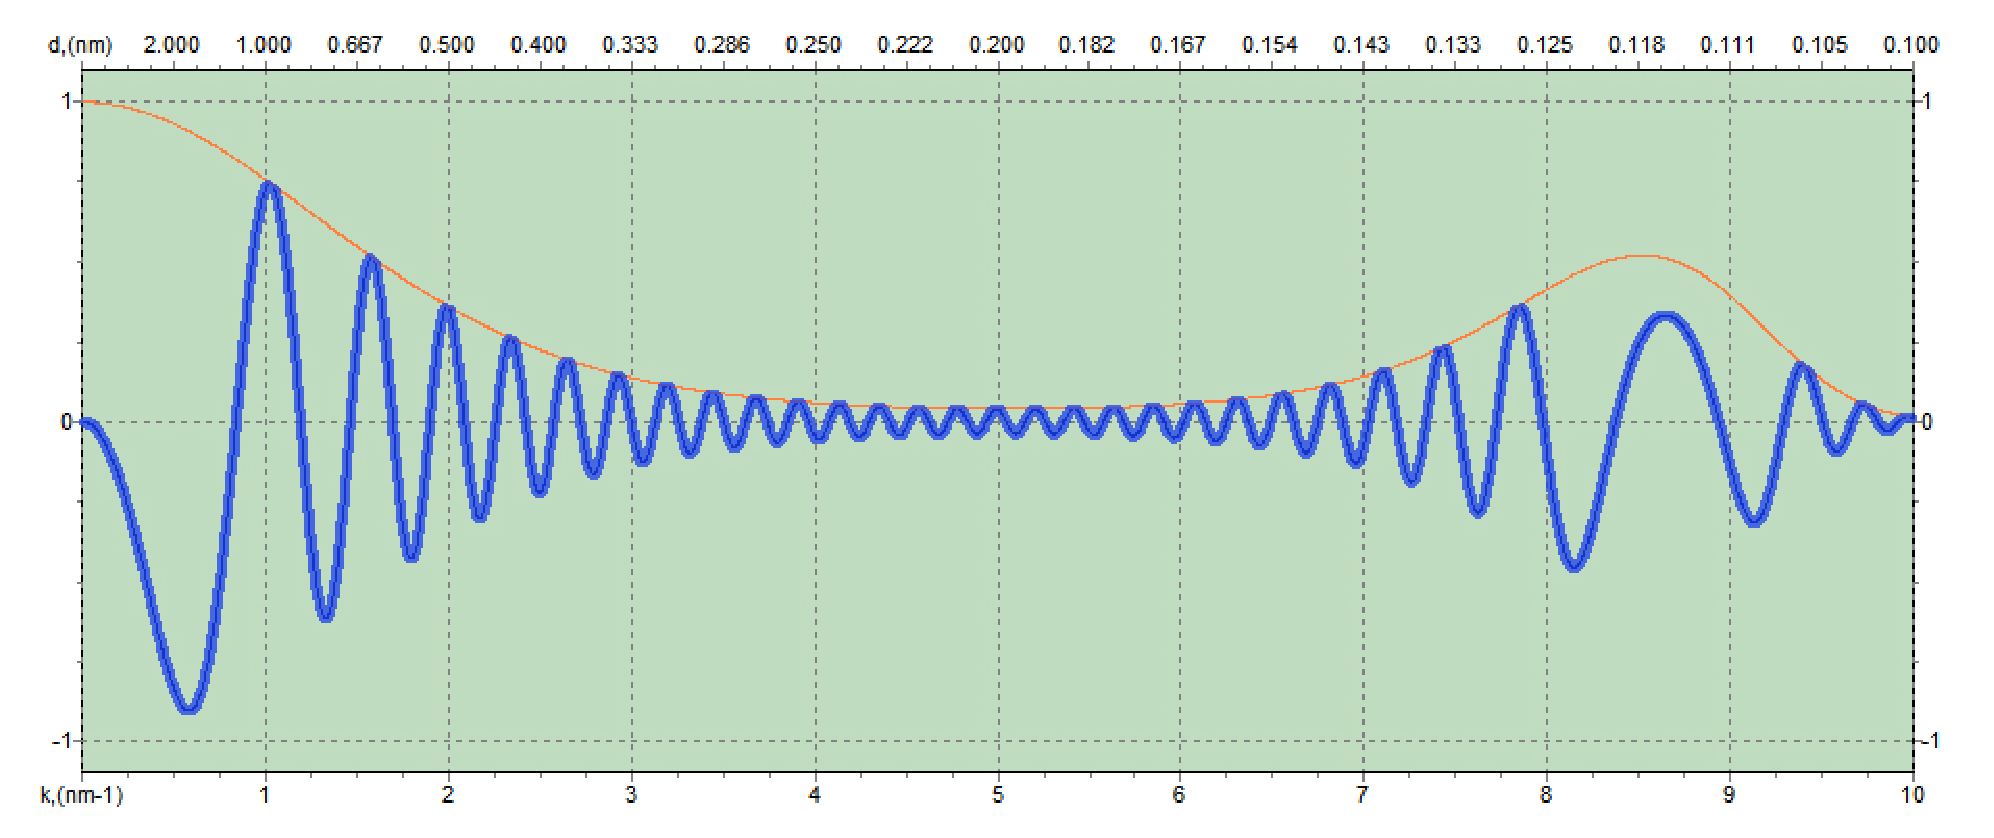
\includegraphics[width=0.5\textwidth]{figures/lichte.pdf}
        \caption{Image showing CTF of a TEM at Lichte defocus}
        \label{fig:ctflichte}
\end{figure}


All of the HRTEM work is preferably done at Scherzer defocus, as it produces most simple to interpret images.
Sometimes `Extended Scherzer', defined as $1.2 \Delta f_{Scherzer}$, is used for HRTEM, where slight linearity is sacrificed to gain more resolution by pushing the resolution limit.
Another important imaging condition is call Lichte defocus.
Described by Hannes Lichte, it is best suitable for holographic reconstructions, as it tried to maximize the information gathered by pushing the decoherence envelope function.\cite{Lichte1991}
Because of large fluctuation in contrast as such (Figure~\ref{fig:ctflichte}), Lichte defocus has little use outside electron holography.
\begin{figure}[t]
    \centering
    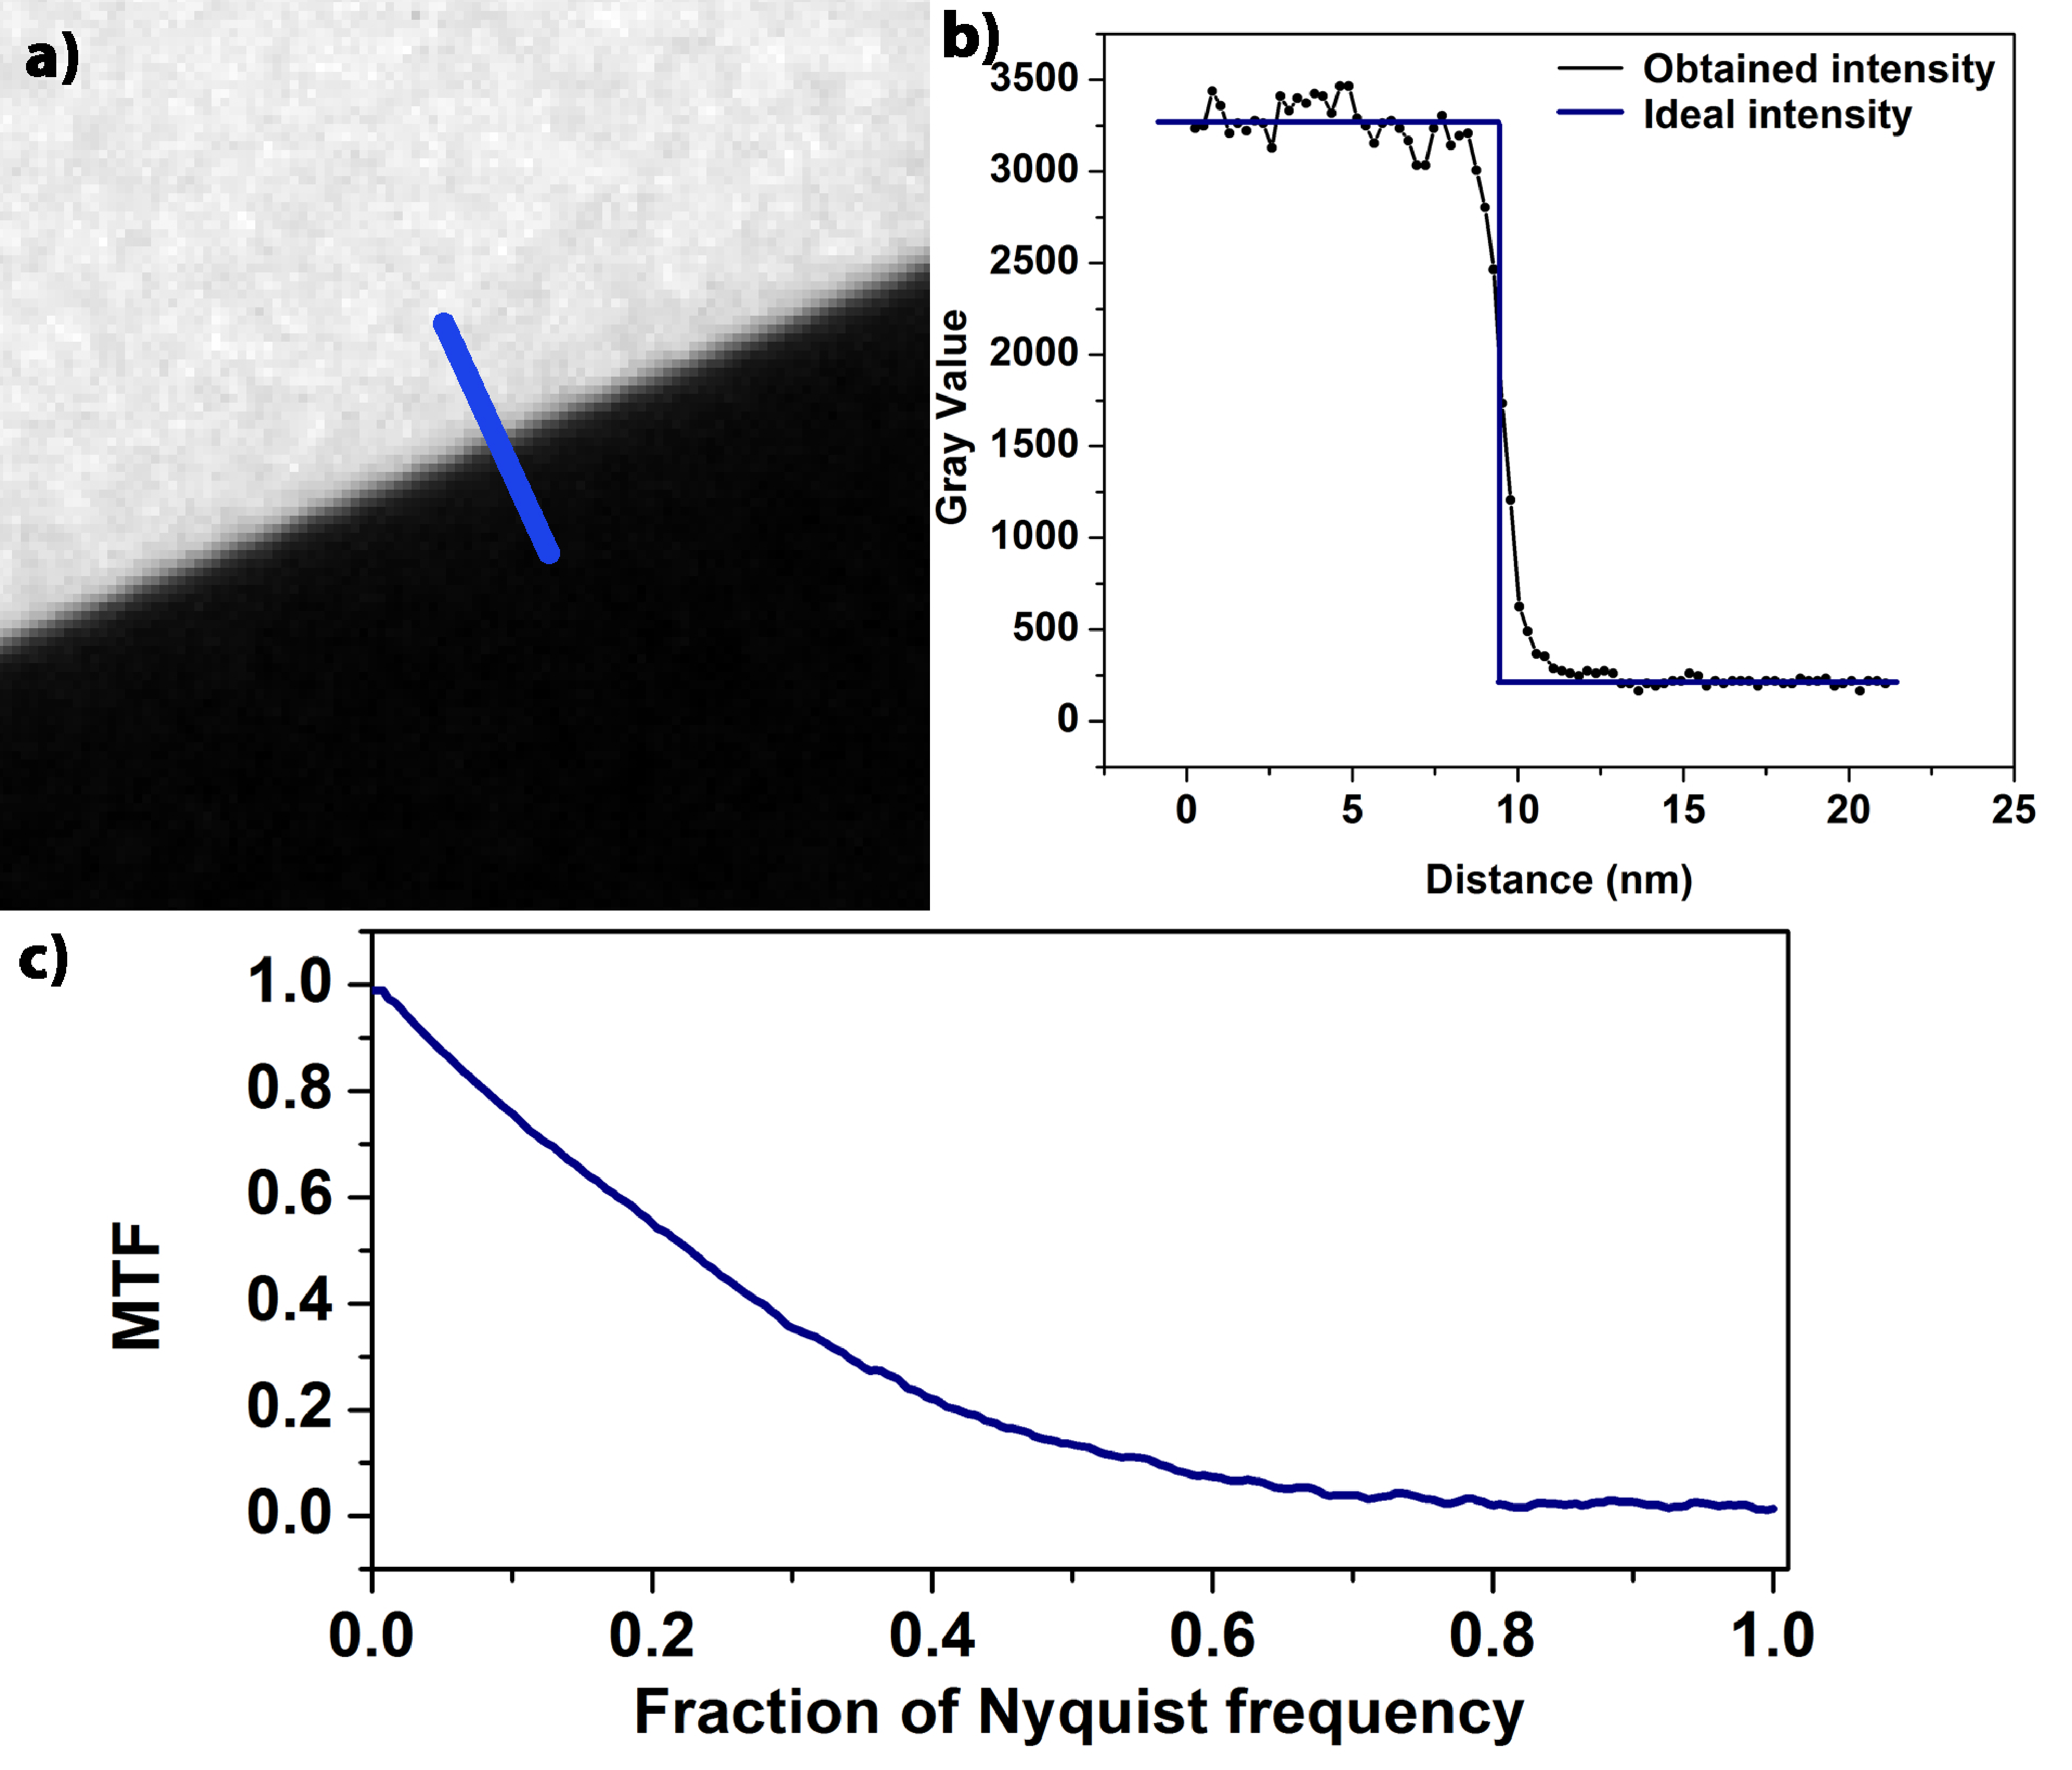
\includegraphics[width=0.9\textwidth]{figures/MTFtheory.pdf}
    \caption{a) A zoomed out image of a shadow of beam blocker, showing diffused edges, b) graphs showing `perfect' edge step function and actual intensity levels along the blue line shown in image (a), and c) MTF of a Olympus-SIS KeenView G2 CCD camera fitted under a JEOL JEM 2100F TEM used in this document (Generated by MTFestimate program, donated generously by Dr. Wouter Van den Broek \cite{VandenBroek2012})}
    \label{fig:mtfall}
\end{figure}

Lichte defocus is given by:
\begin{equation}
    \Delta f_{Lichte} = -\frac{3}{4} C_s (q_{max} \lambda)^2
\end{equation}
Here $q_{max}$ is the maximum spatial frequency till which information is available.
It is limited by objective aperture or information limit.

\subsection{Modulus Transfer Function (MTF)}
Till now we discussed only about the electron microscope and its physical limitations.
Final step in any image acquisition is it image formation on the camera.
For CCD cameras, which are most used ones today, a unique problem arises, that is of transfer of contrast from a periodic image.

In ideal case any camera should be able to record exact intensities from the sample, \textit{i.e.} if we place any opaque object in its path then opaque areas shall be dark or intensity shall be zero, while transparent areas shall be completely bright.
However due to construction of CCD and due to quantization of image in terms of pixels, contrast transfer as such is not perfect and there is a transition zone in which contrast will go from zero to desired value as a sinusoidal function (Figure~\ref{fig:mtfall}a and b).

If we now consider any periodic lattice, which is being imaged, we can see that how the contrast levels of that lattice spacing will depend on the camera (\textit{e.g.} Figure~\ref{fig:mtfexample}).

\begin{figure}[b]
    \centering
    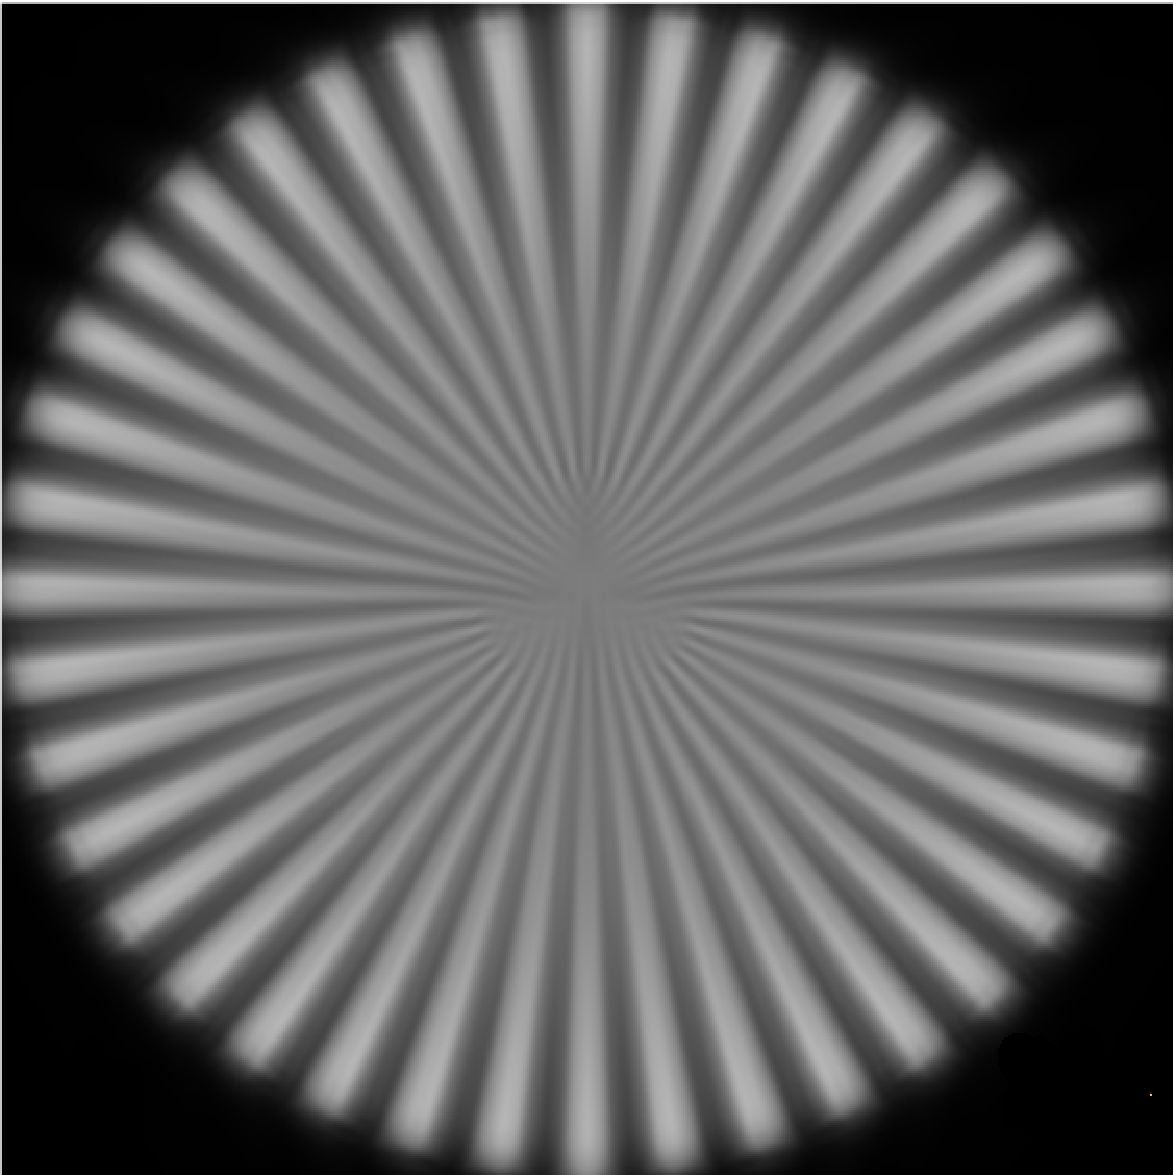
\includegraphics[width=0.30\textwidth]{figures/mtfeg.pdf}
    \caption{An image showing change in contrast of an image recorded on digital camera, as we go from lower spatial frequency to higher spatial frequencies [image credit:Tom.vettenburg, via Wikimedia Commons]}
    \label{fig:mtfexample}
\end{figure}

This relation between the difference in contrast between dark and light fringes for a periodic spacing being imaged is called Modulus Transfer Function or MTF of the camera.
Ideally it should be 1 as all frequencies shall be reproduced with actual contrast, however for an actual camera it looks like as shown in Figure~\ref{fig:mtfall}c.

For further details please consult \cite{VandenBroek2012,Koeck2000}